\section{Initialization}
The particles are placed in a fcc bravais lattice structure. After defining the density $\rho$ and the number of particle $N$, the unit cells are filled. To avoid overlap between unit cells, each unit cell contains 4 particles, as shown in figure %\ref{fig:unit_cell}

% \begin{figure}
% \centering
% 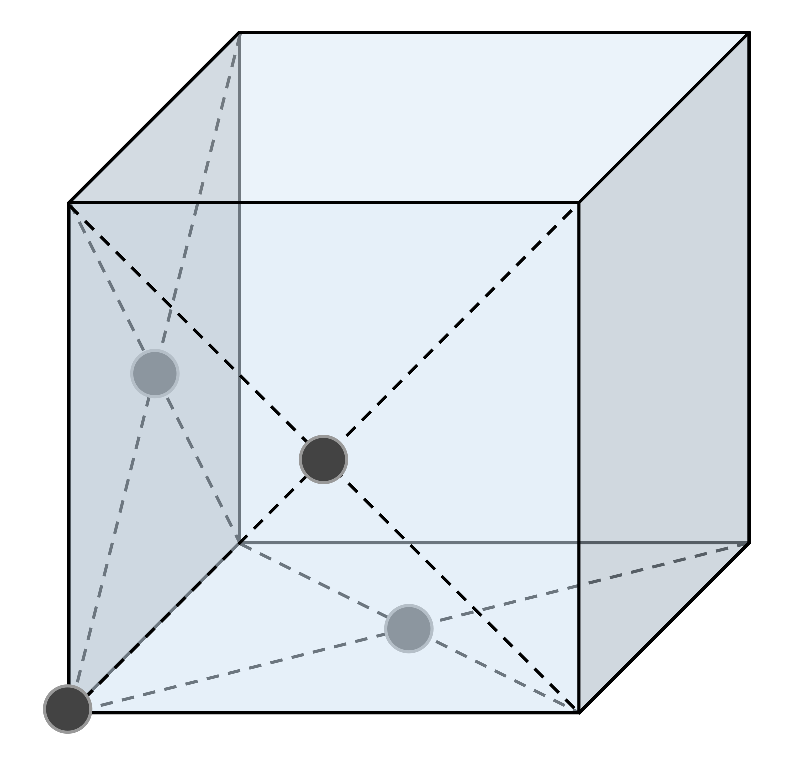
\includegraphics[width=\linewidth]{fcc_cell.eps}
% % \fbox{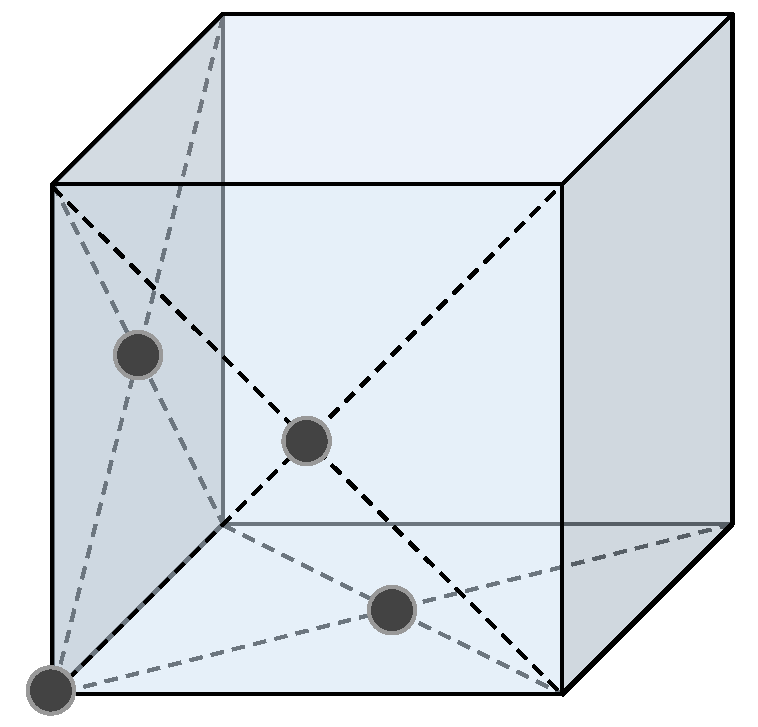
\includegraphics{fcc_cell.pdf}} 
% \caption{Unit cell}
% \label{fig:unit_cell}
% \end{figure}


\begin{Figure}
 \centering
 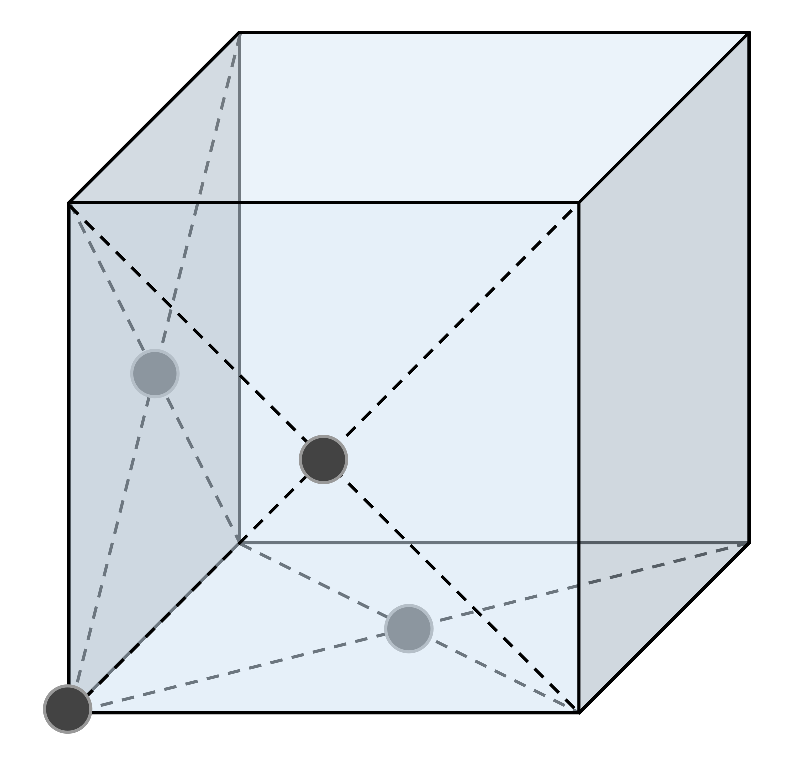
\includegraphics[width=0.5\linewidth]{fcc_cell.eps}
 \captionof{figure}{my caption of the fugure}
\end{Figure}
[[init velocity]]

Lennard-Jones pair potential:
\begin{gather*} 
    U(r) = 4\epsilon\left[\left(\frac{\sigma}{r}\right)^{12}-\left(\frac{\sigma}{r}\right)^6\right].
\end{gather*}